\chapter{Platform Interface}
\label{ch:interface}

The MEDF platform is equipped with an interactive web-based dashboard built using Streamlit. This interface provides a user-friendly environment for analysts, developers, and other stakeholders to conduct ethical evaluations without needing to interact directly with the backend API or the codebase. The dashboard is designed to guide the user through the evaluation workflow, from configuration to results analysis. This chapter describes the critical features and components of the user interface, illustrated with screenshots captured from the live application running on localhost.

\section{Main Evaluation View}
\label{sec:main_view}

The primary view lets the user configure and run a new evaluation by selecting an AI system, setting baseline dimension scores on the 1--7 Likert scale and choosing the frameworks and stakeholder profiles to include in the analysis. A \enquote{Run Demo Scenario} button populates the form with pre-configured case study data to support quick demonstration and testing. Figure~\ref{fig:evaluate_tab} shows the evaluation configuration interface.

\begin{figure}[H]
\centering
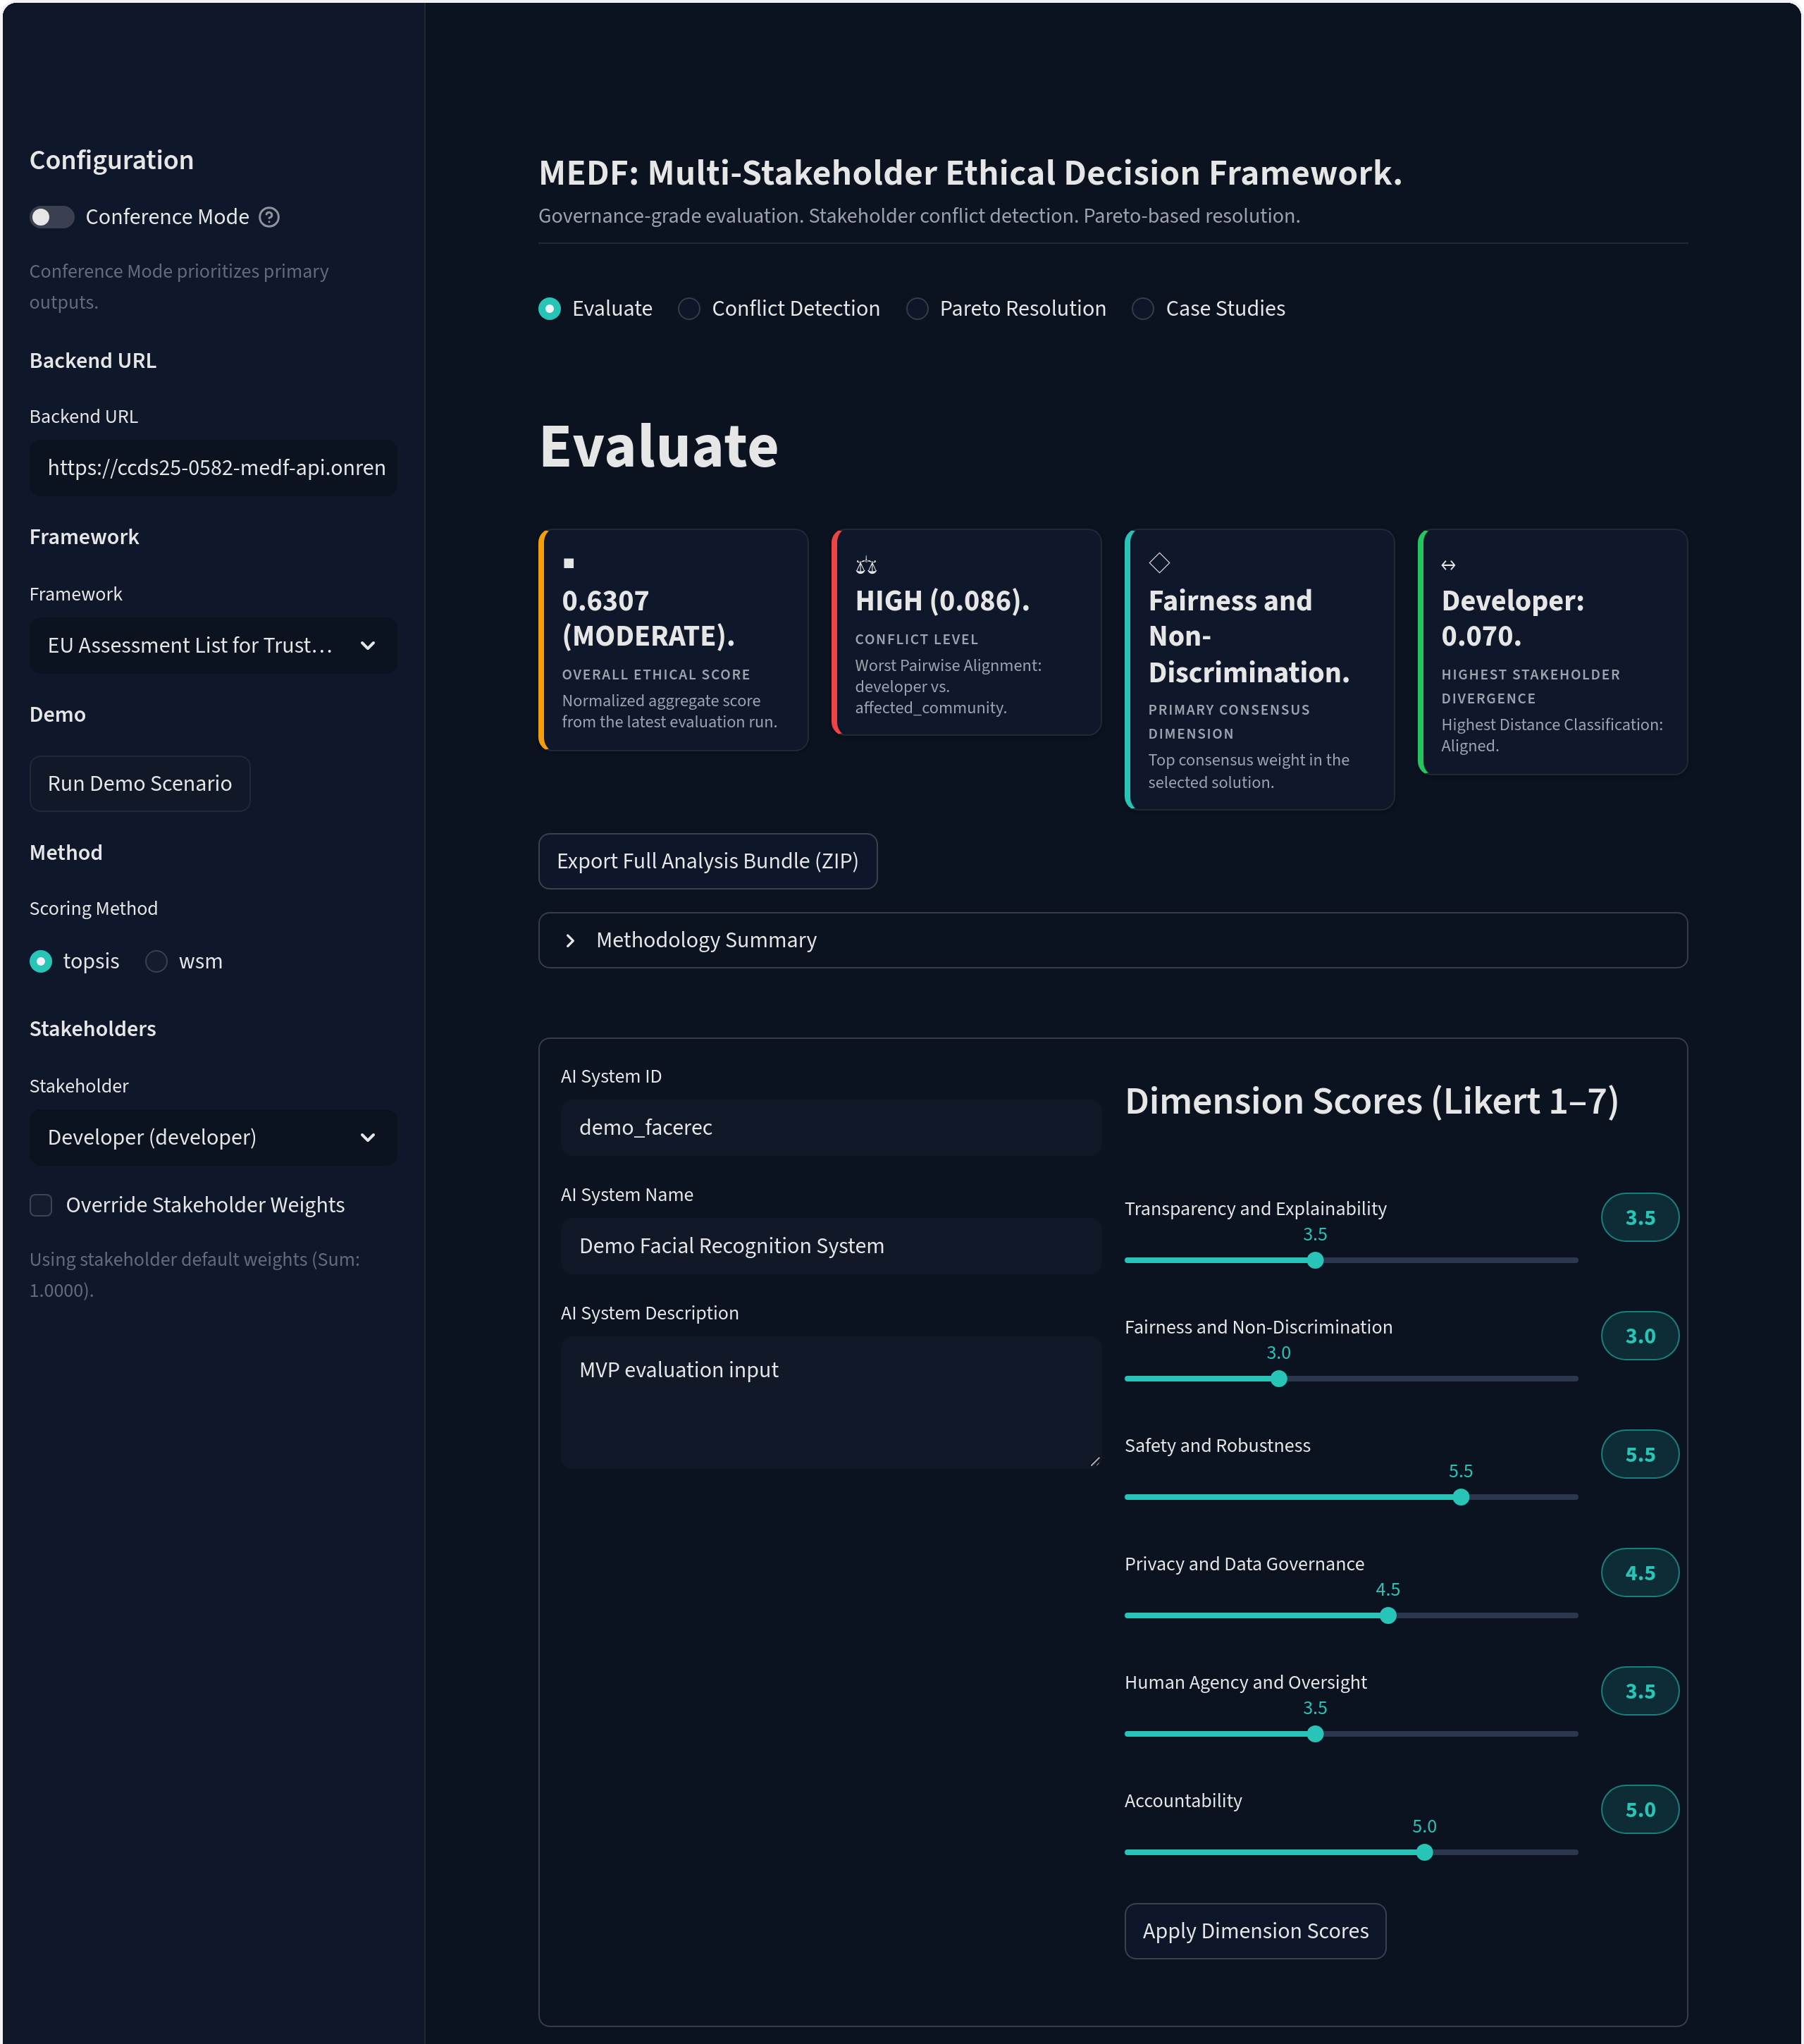
\includegraphics[width=0.95\textwidth]{figures/fig_10_1_evaluate_config.png}
\caption{MEDF evaluation configuration interface showing dimension score sliders, framework selection, and stakeholder weight customization.}
\label{fig:evaluate_tab}
\end{figure}

\section{Results Visualization}
\label{sec:results_viz}

Once an evaluation completes, the dashboard presents the outcome as an overall score gauge (color-coded by risk level), a framework score breakdown bar chart and a dimensional contribution radar chart that surfaces the ethical strengths and weaknesses of the system. Figure~\ref{fig:evaluate_results} shows the evaluation results after running the demo scenario.

\begin{figure}[H]
\centering
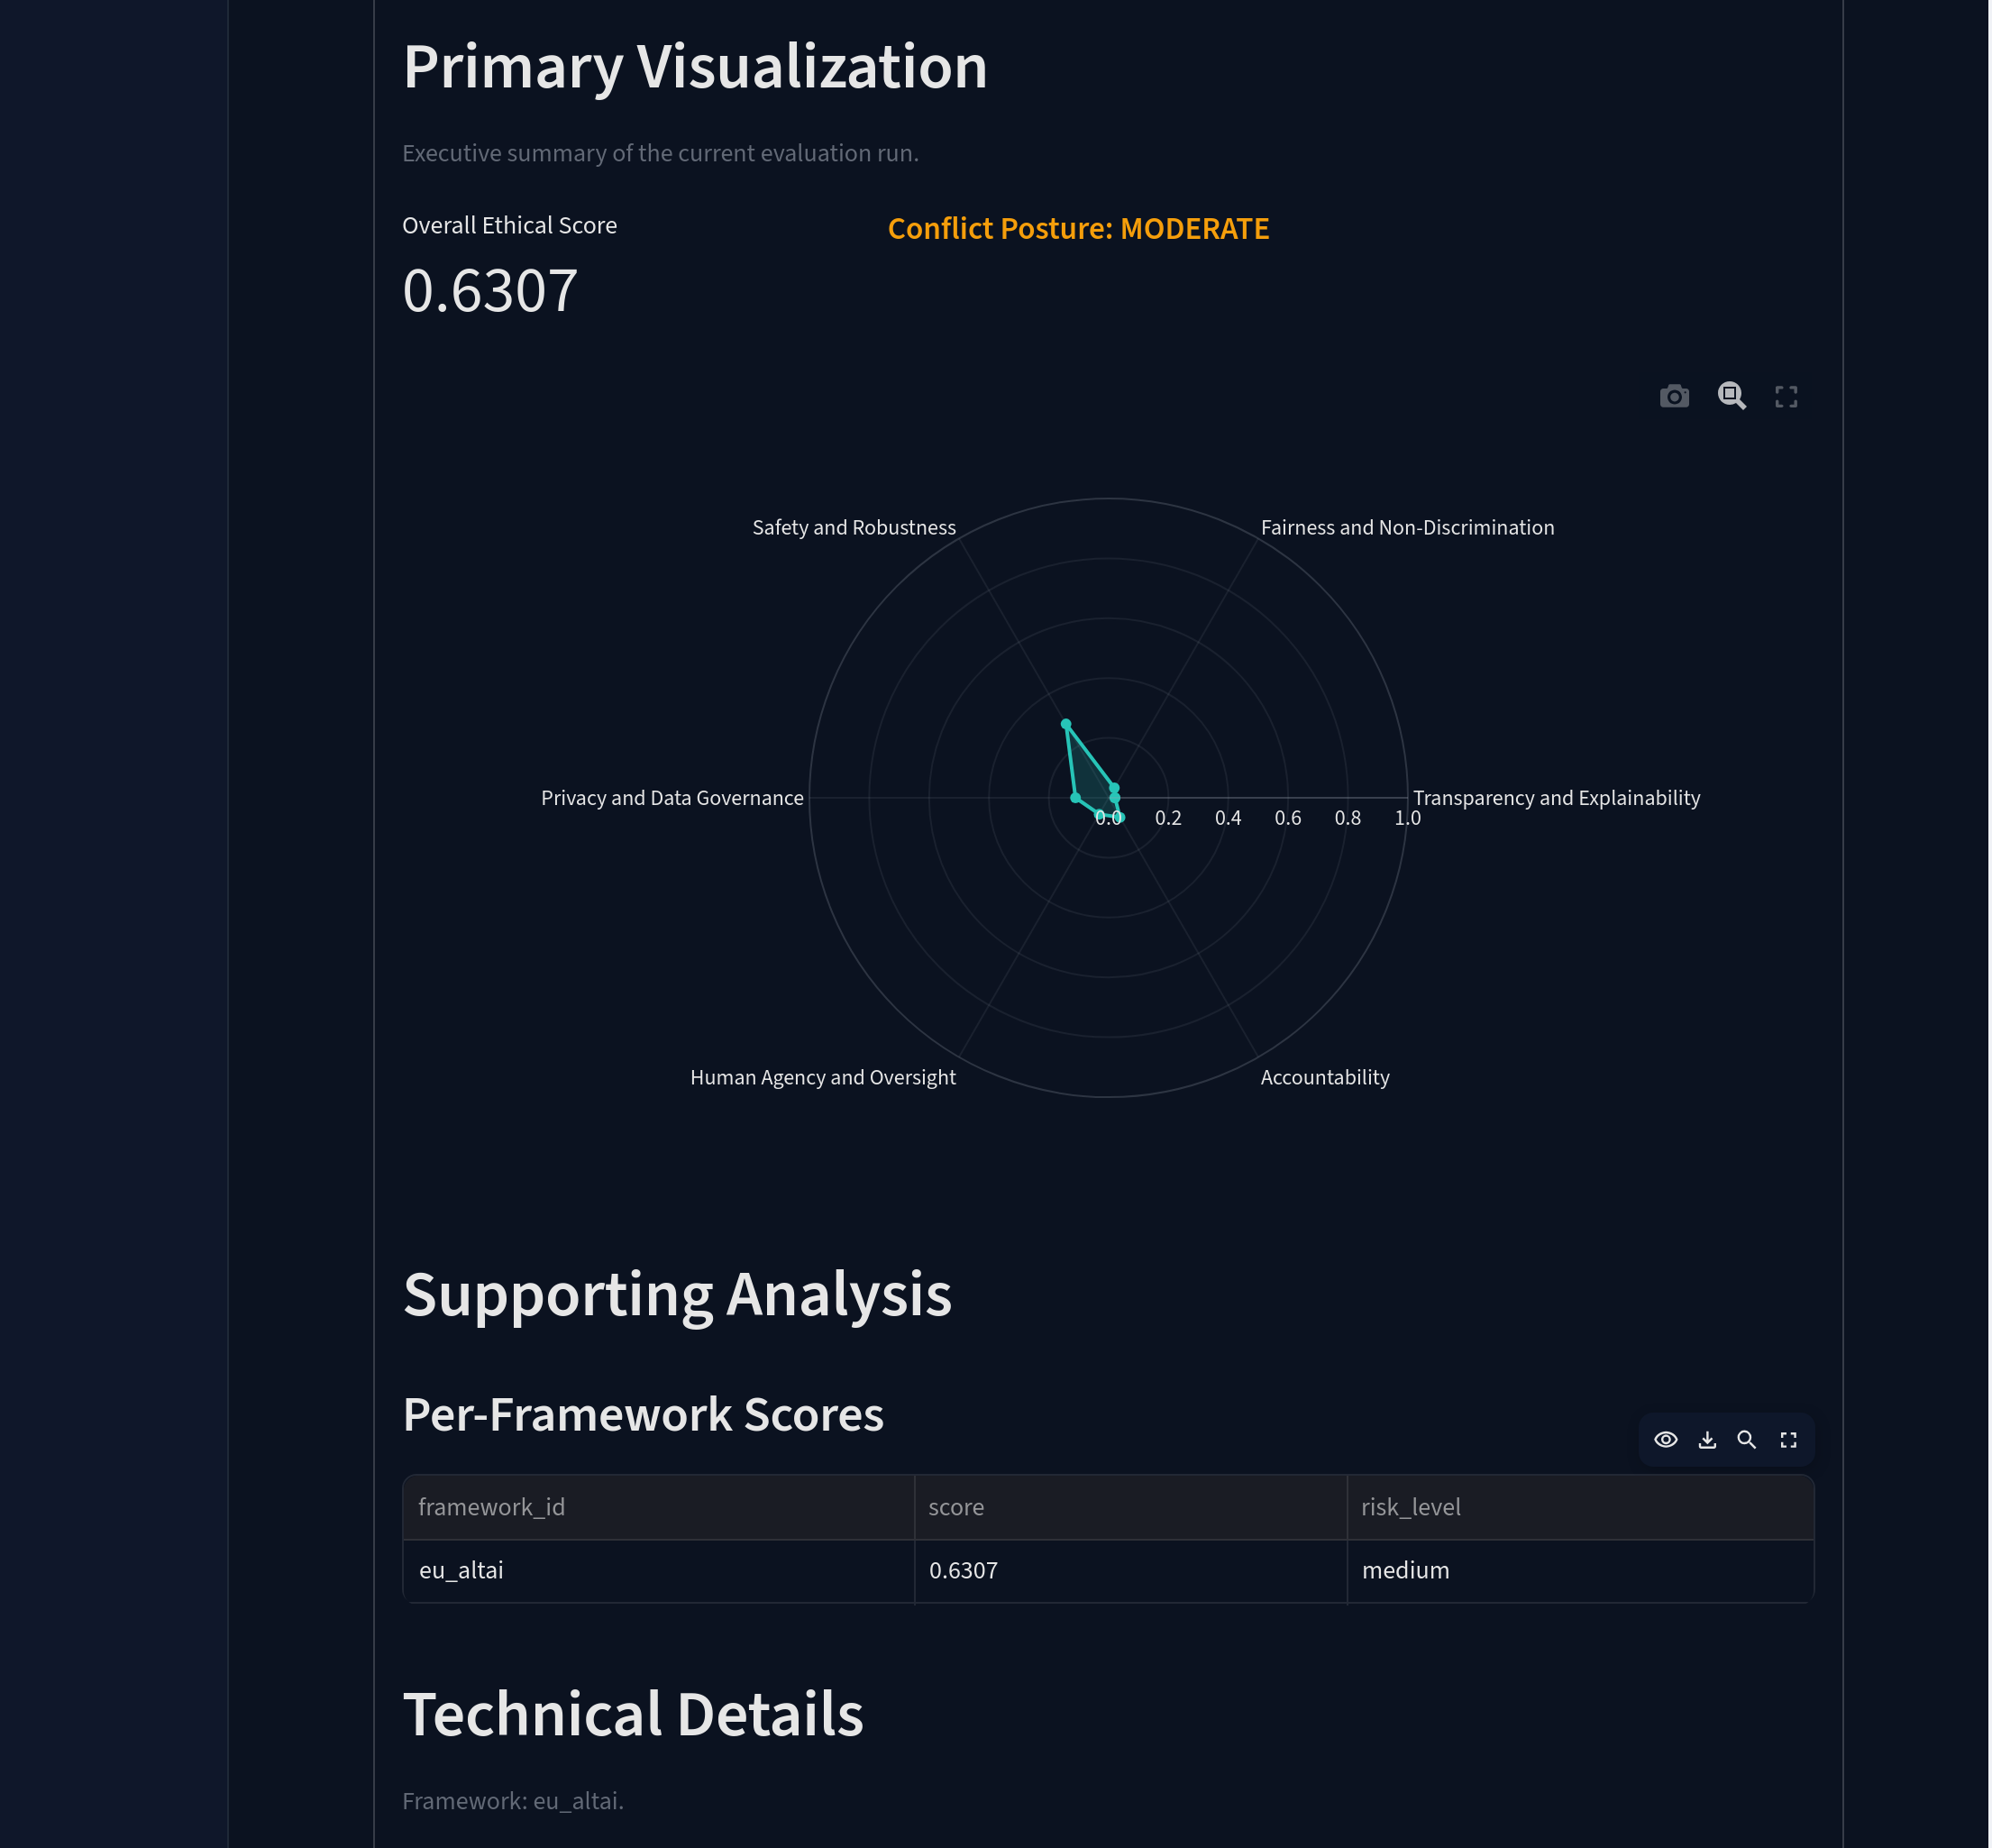
\includegraphics[width=0.95\textwidth]{figures/fig_10_2_results_viz.png}
\caption{MEDF evaluation results showing the overall score, framework breakdown, and dimensional contributions.}
\label{fig:evaluate_results}
\end{figure}

\section{Conflict and Consensus Analysis}
\label{sec:conflict_viz}

The conflict analysis view displays a heatmap of Spearman's rank correlation coefficients between stakeholder pairs and, when Pareto optimization is run, a plot of non-dominated consensus solutions that lets the user visually explore trade-offs between compromise options. Figure~\ref{fig:conflict_tab} shows the conflict detection interface and Figure~\ref{fig:pareto_tab} shows the Pareto resolution interface.

\begin{figure}[H]
\centering
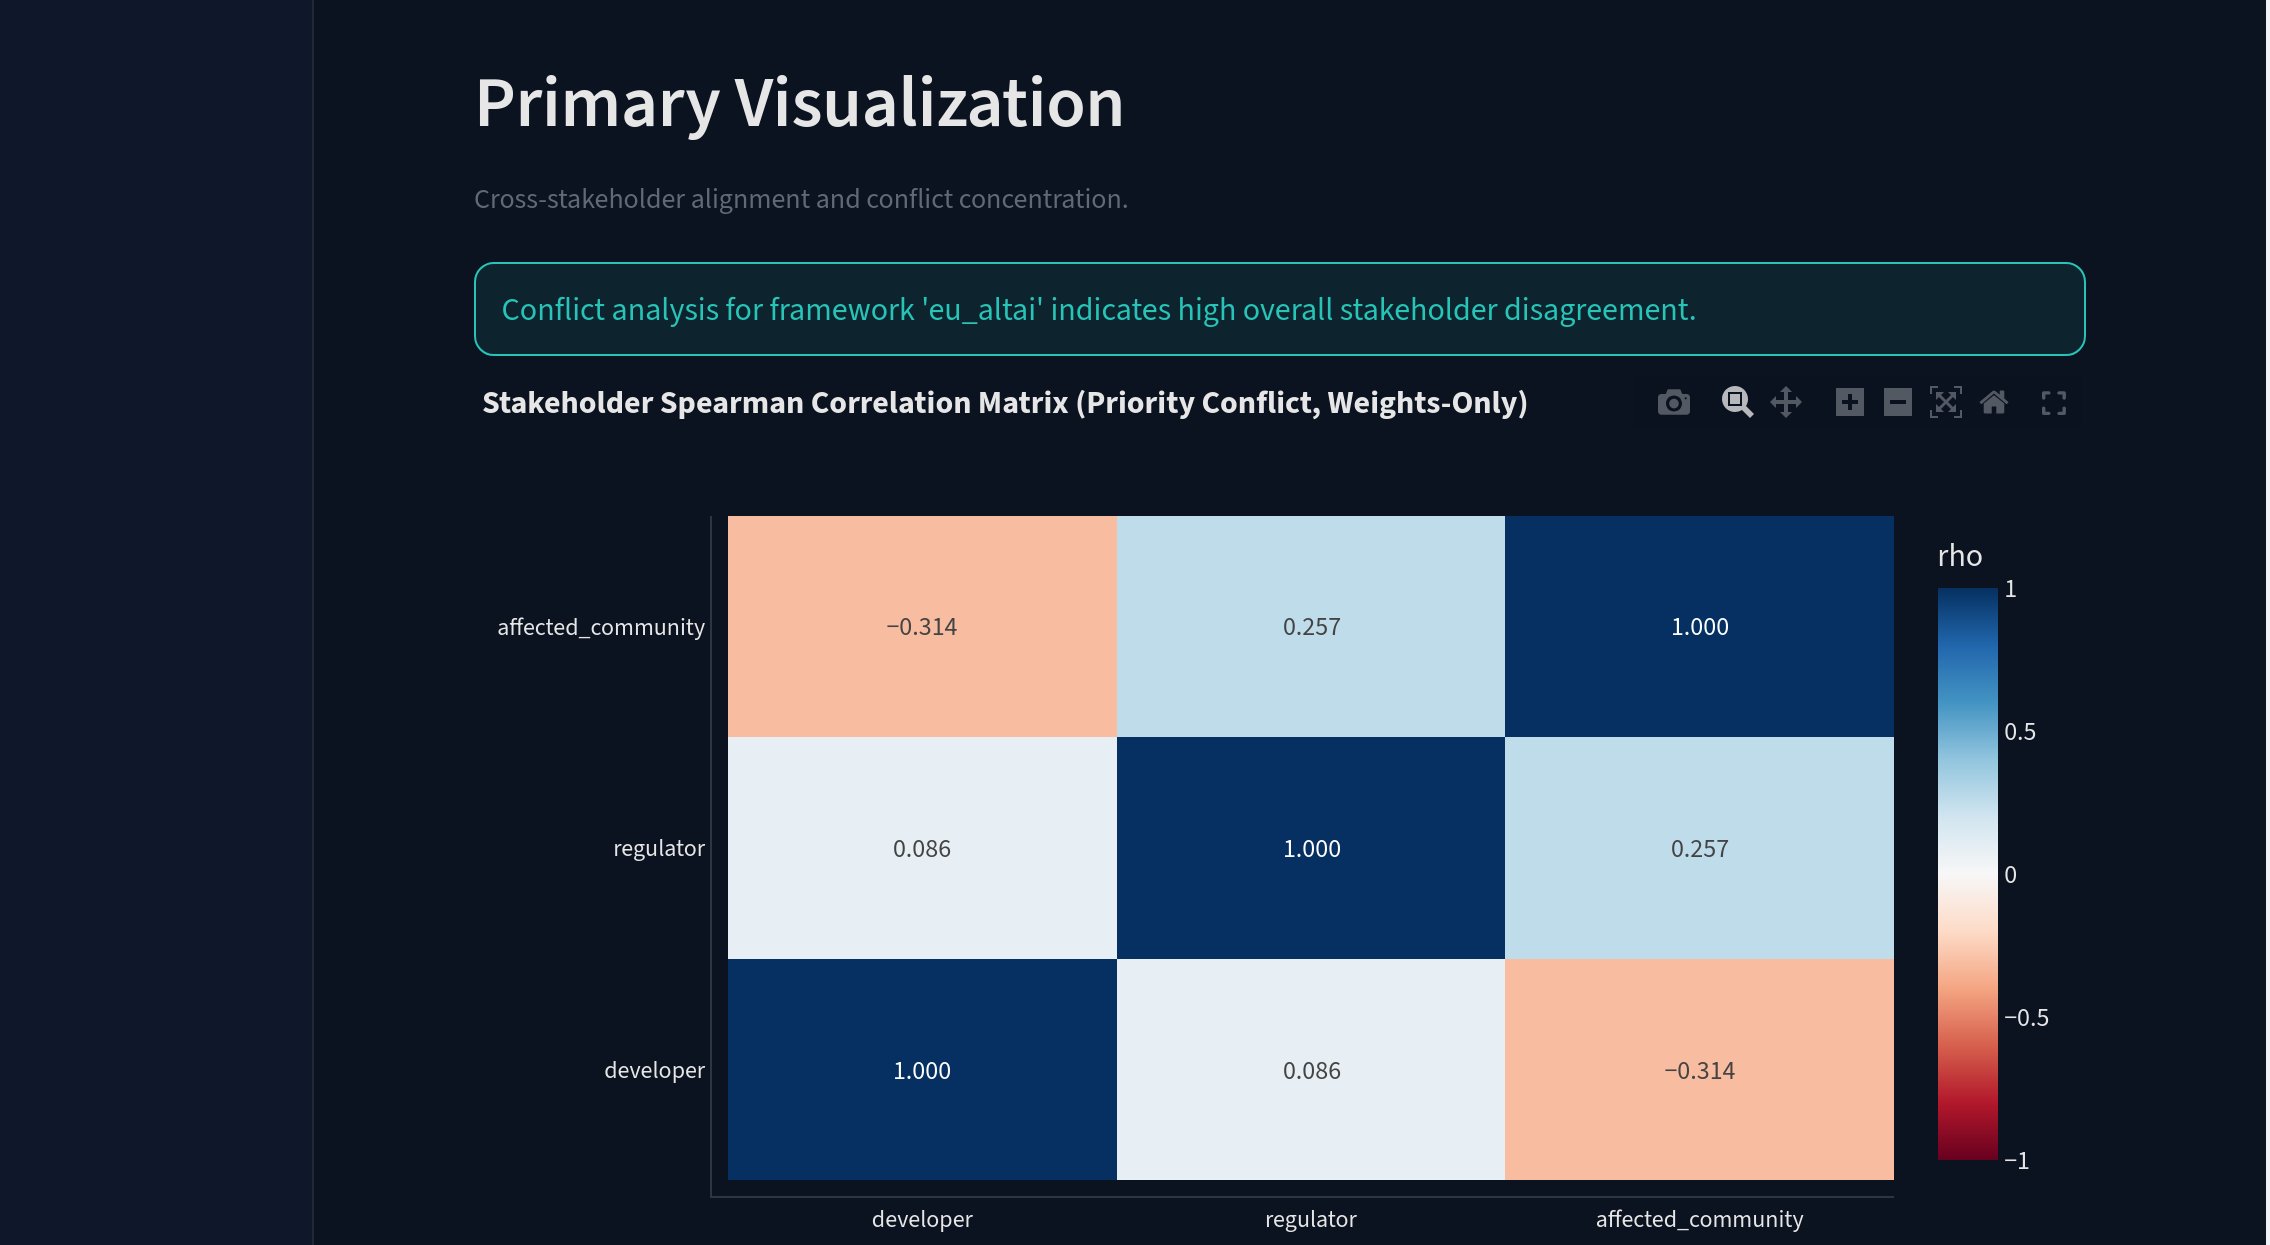
\includegraphics[width=0.95\textwidth]{figures/fig_10_3_conflict_heatmap.png}
\caption{Conflict detection interface showing the stakeholder conflict matrix heatmap.}
\label{fig:conflict_tab}
\end{figure}

\begin{figure}[H]
\centering
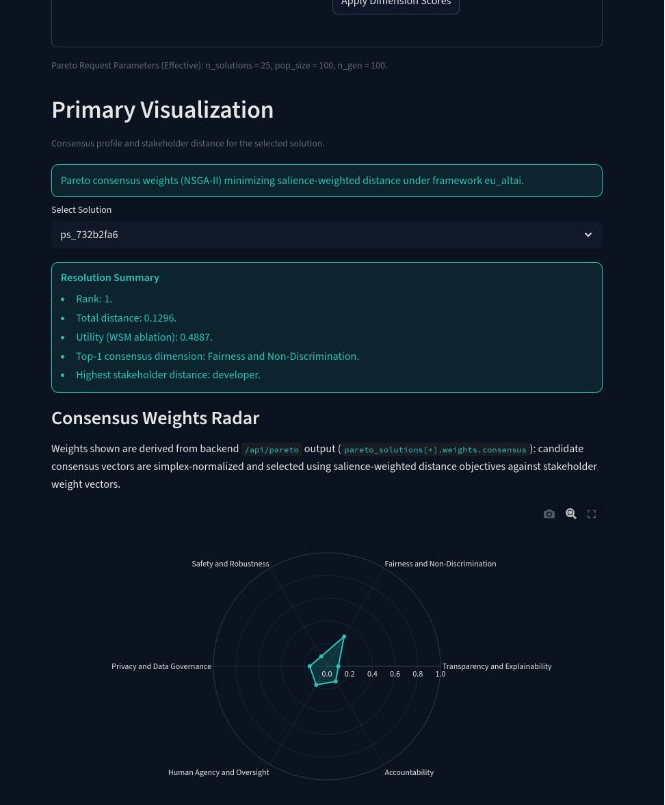
\includegraphics[width=0.95\textwidth]{figures/fig_10_4_pareto_resolution.png}
\caption{Pareto resolution interface showing the consensus optimization results.}
\label{fig:pareto_tab}
\end{figure}

\section{Case Study Browser}
\label{sec:case_browser}

The Case Studies tab lets the user browse and run the three pre-configured case studies (Facial Recognition, Hiring Algorithm, Healthcare Diagnostic), each displayed with a system summary, deployment context, known risks and evidence sources, with a single click triggering a complete evaluation to reproduce the results in Chapter~\ref{ch:case_studies}. Figure~\ref{fig:casestudies_tab} shows the case study browser, and Figure~\ref{fig:casestudy_results} shows the results after running Case Study~1.

\begin{figure}[H]
\centering
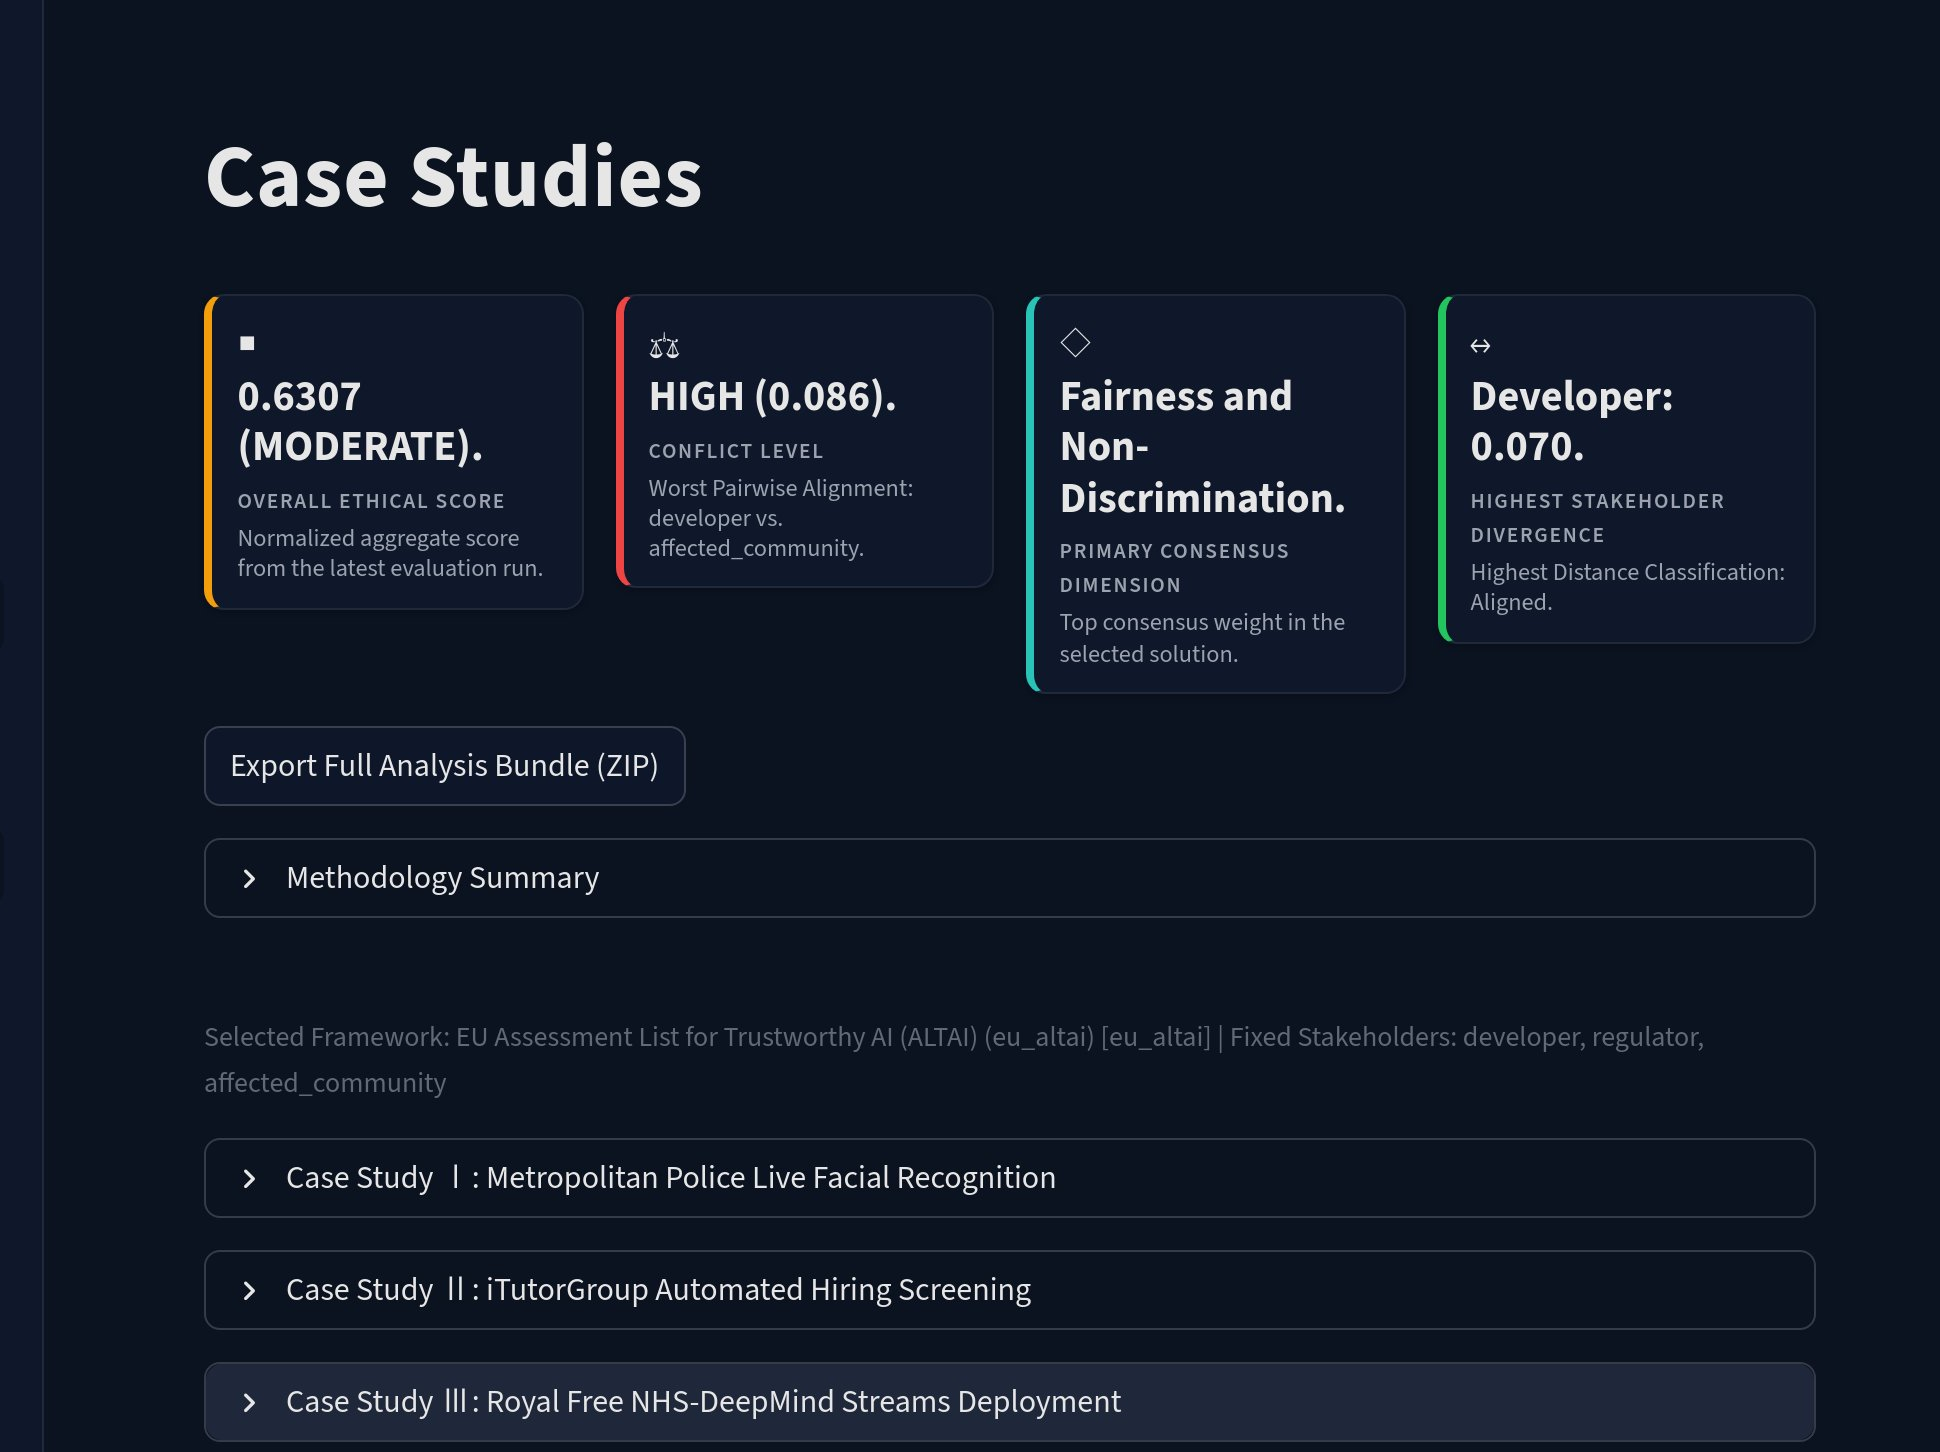
\includegraphics[width=0.95\textwidth]{figures/fig_10_5_case_study_browser.png}
\caption{Case study browser showing the three pre-configured case studies with system descriptions and evidence sources.}
\label{fig:casestudies_tab}
\end{figure}

\begin{figure}[H]
\centering
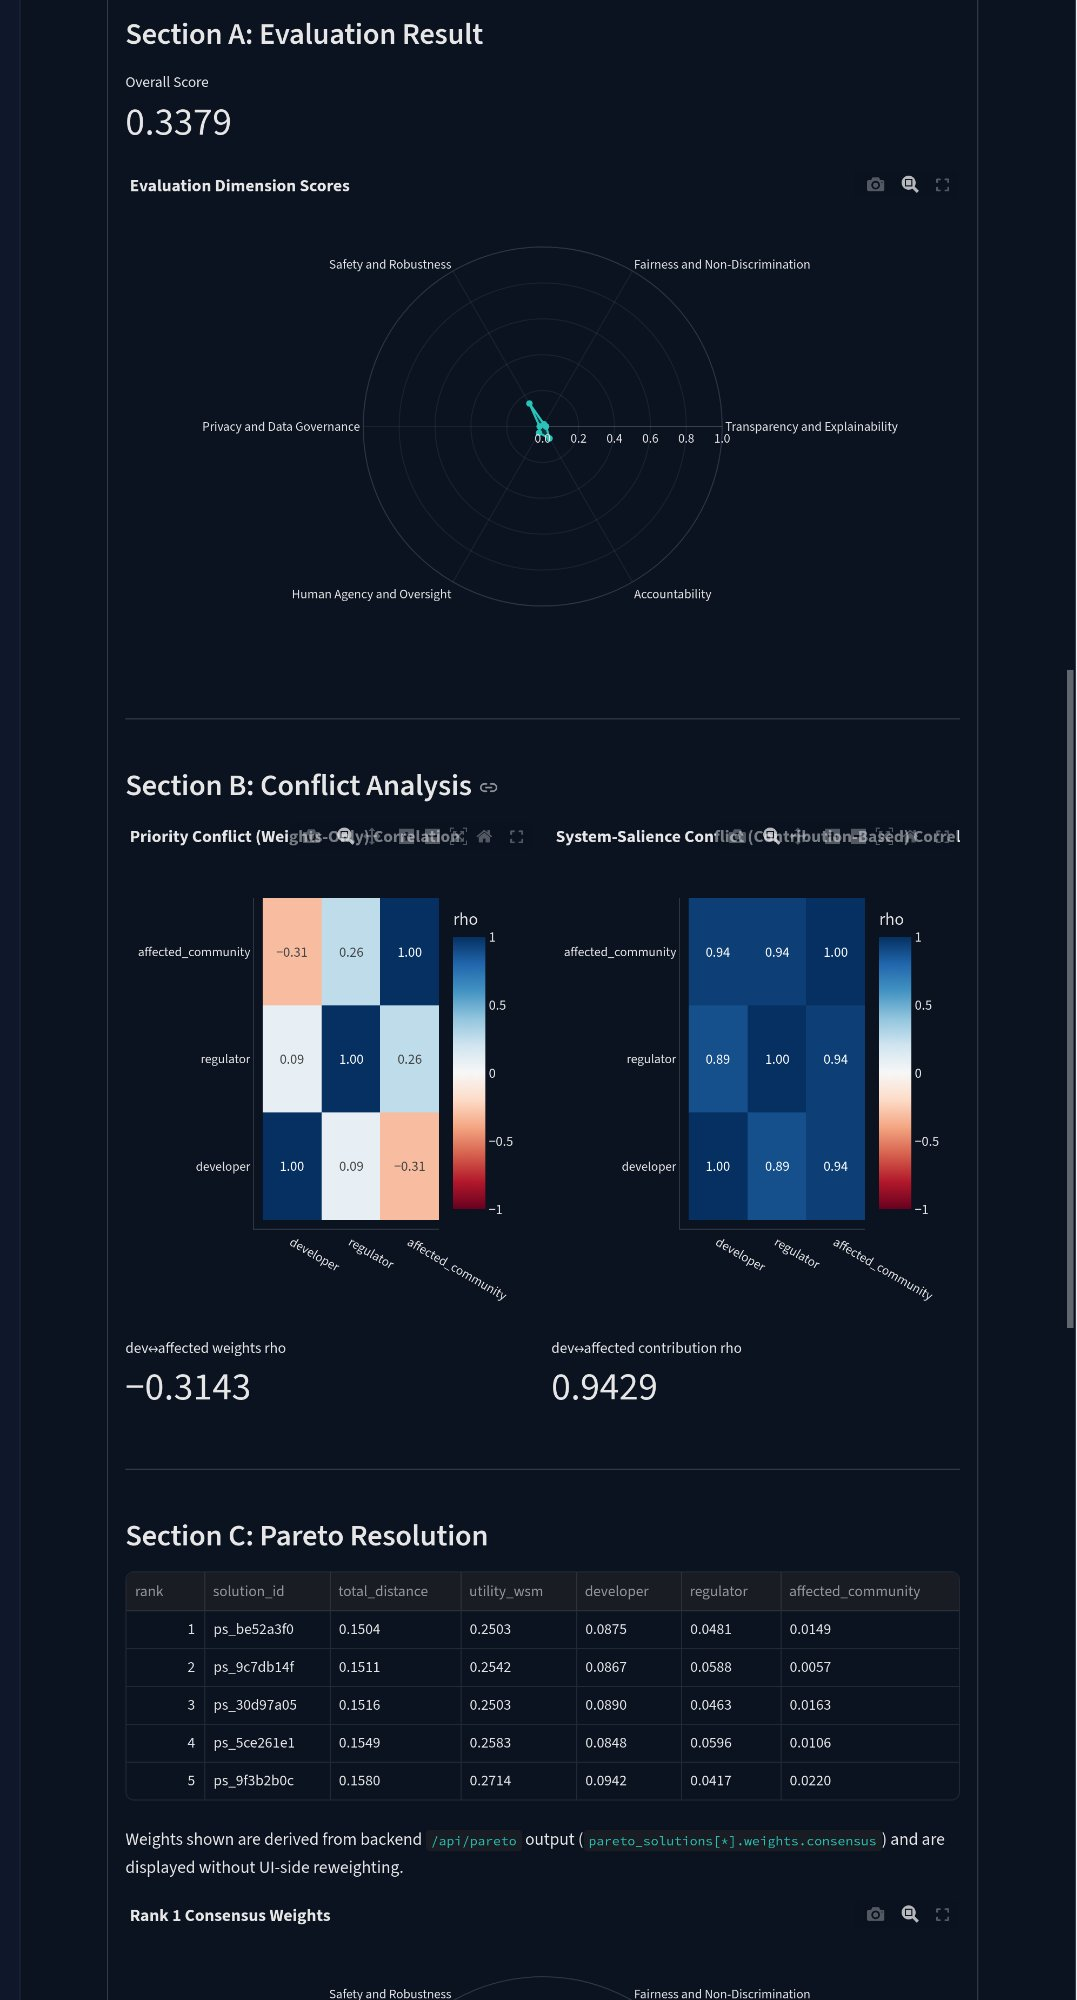
\includegraphics[width=0.95\textwidth]{figures/fig_10_6_case_study_1_results.png}
\caption{Case Study 1 (Facial Recognition) evaluation results showing the overall score of 0.3379 and per-stakeholder breakdown.}
\label{fig:casestudy_results}
\end{figure}

By providing these interactive visualizations, the Streamlit dashboard makes the complex, multi-dimensional results of the MEDF evaluation accessible and interpretable for a non-technical audience, facilitating a more informed and data-driven discussion about AI ethics.
